\section{CPSs as Multi-agent systems}
In this second part we will consider \textbf{Cyber-physical systems} as \textbf{multiagent systems} which in general can be modeled by using a directed graph (\textbf{digraph}). The figure below is an example:

\begin{figure}[h]
    \centering
    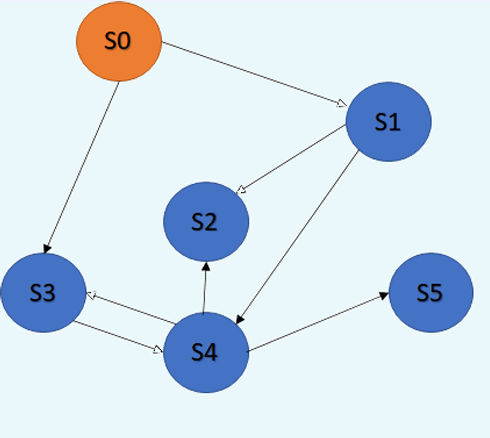
\includegraphics[scale=0.6]{images/MultiAgent.png}
    \caption{A digraph describing a multi-agent CPS}
\end{figure}

Each agent, denoted with $S_i$, can be thought as an LTI dynamical system, furthermore the digraph is used in order to represent  the \textbf{communication} among the agents which compose the \textit{overall system}.\\
In this particular \textbf{framework of multi-agent CPSs} two control problems can be recognized:
\begin{itemize}
    \itemsep0em
    \item {\color{blue}\textbf{Cooperative Tracking problem}} in which there is one \textbf{leader node}, denoted with $S_0$ and the remaing part of the nodes are N other \textbf{identical agents} which are the so-called \textbf{follower nodes}; in this type of control setting the agents \textit{cooperate} in order to follow a reference \textit{dictated by the leader node}. Examples of this approach can be: platooning, formation control and so on. {\color{red}We will focus our attention mainly on this one...} 
    \item {\color{blue}\textbf{Cooperative synchronization problem}}, the cooperation is also here in order to reach a Consensus, but in this case there is an \textbf{absence of a leader node}.
\end{itemize} 

Starting from this point we have to do an \textbf{assumption} in order to develop properly the theory:
\begin{quotation}
    \color{red}
    \textbf{Assumption} The N agents of the multi-agent system describing the CPS are \textbf{identical}, including the leader.
\end{quotation}
More later through the discussion on these topics, we will exploit a trick in order to generalize as much as possible the description of this framework.

\section{Review of LTI systems structural properties}
\noindent
Before to start talking about control algorithms and protocols can be used in the framework of multi-agent systems, it is better to retrieve and/or introduce some notions which are particularly important:
\begin{enumerate}
    \item At first a mathematical structure for the agents will be assumed (LTI systems) and some specific \textbf{structural properties} will be reminded;
    \item Then some notions on \textbf{How we can derive the mathematical model of the agents} will be given in the general framework of \textbf{black-box Error-In-Variables (EIV) System Identification}
\end{enumerate}

At the moment we can assume that the structure of the dynamical system associated to each agent $S_i$ is the Linear Time Invariant (LTI) one. Then, we can say that in the framework of \textbf{Cooperative Tracking Problem} holds that:
\begin{enumerate}
    \item The \textbf{leader node} $S_0$ is the following, at the moment we will consider that on the leader node no input is applied 
    \begin{equation}
        \begin{aligned}
            S_0: \ \begin{cases}
                \dot{x}_0=Ax_0\\
                y_0=Cx_0
            \end{cases}
        \end{aligned}
    \end{equation}
    \item The \textbf{follower nodes} $S_i, \ i=1,..., N$ are modeled as 
    \begin{equation}
        \begin{aligned}
            S_i=\begin{cases}
                \dot{x}_i=Ax_i+Bu_i\\
                y_i=Cx_i
            \end{cases}
        \end{aligned}
    \end{equation}
\end{enumerate}

At this point it is important to assume that \textbf{the triple} $(A, B, C)$ is \textbf{stabilizable} and \textbf{detectable}. 
Let us remind these important \textbf{structural properties} these dynamical systems.

\subsection{Controllabilty of an LTI system}
Roughly speaking we can say that a system is \textbf{completely (or fully) controllable} if one can \textbf{impose the behaviour} of \textbf{ALL the state variables} 'only' by acting on the inputs.  \\
Practically speaking if the system is \textit{fully controllable} then we are able to design a \textbf{state feedback} controller $K$ which is able to assign to the matrix $A-BK$ an \textbf{arbitrary} selected set of eigenvalues. We are applying to the system the law control input
\begin{equation}
    u=-Kx+\alpha r
\end{equation}

\begin{figure}[h]
    \centering
    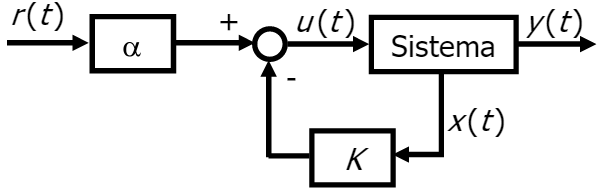
\includegraphics[scale=0.8]{images/state_feedback.png}
\end{figure}

\hspace*{-5mm}
\begin{tikzpicture}
\node [mybox] (box){%
    \begin{minipage}{.96\textwidth}     %Larghezza del box
            {\large{
                \textbf{Result (Controllability)}\\
                An LTI system is \textbf{fully controllable} if and only if the \textbf{controllability matrix} defined as following
                \begin{equation}
                    M_r=\big[ B \quad 
                    AB \quad A^2B \quad \dots
                    \quad A^{n-b}B
                    \big], \quad b=rank(B)
                \end{equation}
                is such that $$\text{rank}(M_r)=n$$
                \noindent
                We can impose to the resulting closed-loop system arbitrary eigenvalues.
            }}
    \end{minipage}
};
\end{tikzpicture}%

\vspace{0.2cm} \noindent
\textbf{What happens if the system is not fully controllable}? This is equivalent to state that rank($M_r$)=$\rho<n$ and so we can only impose $\rho$ out of $n$ eigenvalues by design a proper state feeedback matrix $K$, while $n-\rho$ eigenvalues cannot be modified. Two major situations can occur:
\begin{itemize}
    \item[(A)] The $n-\rho$ eigenvalues have \textit{real part} which is strictly negative $\iff$ the system is {\color{red}\textbf{stabilizable}  }.
    \item[(B)] The remaining $n-\rho$ eigenvalues have real part which is greater or equal than zero $\iff$ the system is \textbf{not stabilizable}.
\end{itemize}

\noindent
We have just understood that when the fully controllability property is not respected the LTI system $\mathcal{S}$ can be divided into two parts:
{\large{
    \begin{equation*}
        \mathcal{S}=\begin{cases}
            \text{controllable part }&\to {\rho \ \text{eigenvalues}}\\
            \text{non-controllable part}&\to {n-\rho \ \text{eigenvalues}}
        \end{cases}
    \end{equation*}
}}

\subsection{Observability of an LTI system}
Roughly speaking we can say that an LTI system is \textbf{completely (or fully) observable} if and only if the behaviour  of \textit{all the state variables} can be \textbf{reconstructed} by only measuring the outputs. This is equivalent to state that \textbf{each variable has an effect on the output}.\\
Practically speaking, if the system if \textit{fully observable}, then we can \underline{always} design a device called (in general) \textbf{Luemberger Observer} which is able to provide an \textbf{estimate} asymptotically convergent of all the state variables by only \textbf{exploiting the information} provided by the inputs and the outputs.  

\begin{figure}[h]
    \centering
    \includegraphics[scale=0.8]{images/observer.png}
\end{figure}

Then, the \textbf{observer} is useful for  designing a feedback controller when we can only measure $y$ and not the entire \textbf{state vector}.
In order to be more specific, on such aspect, if the system is \textbf{fully observable}, then we can always find the \textbf{observer gain matrix} $L$, to arbitrarily assign the eigenvalues of the matrix $A-LC$, which describe the dynamics of the \textbf{estimation error}. \\

\hspace*{-5mm}
\begin{tikzpicture}
\node [mybox] (box){%
    \begin{minipage}{.96\textwidth}     %Larghezza del box
           {\large{
            \textbf{Result(Observability)}\\
            An LTI system is \textbf{fully observable} if and only if the \textbf{observability matrix} defined as following
            \begin{equation}
                M_o=\begin{bmatrix}
                    C\\CA\\\vdots\\C^{n-c}A
                \end{bmatrix}, \ c=rank(C)
            \end{equation}
            is such that 
            $$\text{rank}(M_O)=n$$
            We can impose to the matrix $A-LC$ a set of eigenvalues which affect the dynamic of the \textbf{estimation error}.
           }}
    \end{minipage}
};
\end{tikzpicture}%

\vspace{0.2cm}
\noindent
\textbf{What is happening if the system is not fully observable?} For sure we can state that rank($M_O$)=$\gamma<n$, so we can impose only $\gamma$ eigenvalues to the matrix $A-LC$. \\
The remaining $n-\gamma$ eigenvalues can be such that:
\begin{itemize}
    \item[(A)] Their real part is \textbf{strictly negative}, in this case we say that the system is {\color{red}\textbf{detectable}}. Otherwise
    \item[(B)] If at least one eigenvalue, among the $n-\gamma$ which are not observable, is null or positive, the system is \textbf{not detectable}.
\end{itemize} 
Similarly than the controllability, also in this case we can decompose the system into two other parts:
{\large{
    \begin{equation*}
        \mathcal{S}=\begin{cases}
            \text{observable part }&\to {\rho \ \text{eigenvalues}}\\
            \text{non-observable part}&\to {n-\rho \ \text{eigenvalues}}
        \end{cases}
    \end{equation*}
}}
\noindent
It is important to remember that:
\begin{quote}
    \color{red}
    Any control technique can work only with the parts \textbf{controllable} and \textbf{observable} of the system $\mathcal{S}$. The remaining \textit{non-observable} and \textit{non-controllable} part have to be \textbf{asymptotically stable}, otherwise whatever is the control method used, those part cannot be modified.
\end{quote}



\noindent
{\color{blue}\textbf{Remark (Transfer function description)}}  Note that we are focusing on the \textbf{state-space description} because the tractation we will do is essentially based on this type of model, BUT without loss of generalities, we might use also the description by mean of the \textbf{transfer function}. Because:
\begin{enumerate}
    \item If the system $\mathcal{S}$ is fully observable and controllable, the \textbf{poles} of the transfer function $H(s)$ or $H(z)$ are the eigenvalues of the system;
    \item If the system is neither fully observable nor controllable, the \textbf{poles of the transfer function} are a subset of the eigenvalues of the system, and in particular whose related to the controllable and observable part.
\end{enumerate}
We can obtain from the state-space representation the transfer function directly by applying the \textbf{Laplace transform}, the inverse step can be done by using the properties of the \textbf{realizability theory}, this frees us to use other types of techniques frequency-based  such as \textit{loop-shaping}, LQR, $\mathcal{H}_\infty$ synthesis and so on.

\section{The communication network through a digraph}
\noindent
We have mentioned that the communication among the agents is modeled by mean of a directed graph. Let us give some more details which are useful when some control algorithms and synchronization protocols are formalized.\\
\noindent
The communication network among the agents is represented by the digraph
{\large{
    \begin{equation}
        \mathcal{G} = \{\mathcal{V}, \mathcal{E}\}, \ \mathcal{V}=\{v_1, v_2, ..., v_N\}, \ 
        \mathcal{E} \subset \mathcal{V} \times \mathcal{V}
    \end{equation}
}}
However, when we treat the \textbf{synchronization problem} it is useful include in the vertices set $\mathcal{V}$ also the vertex associated to the \textit{leader node} obtaining an \textbf{augmented graph}
{\large{
    \begin{equation}
        \bar{\mathcal{G}} = \{
            \bar{\mathcal{V}}, \bar{\mathcal{E}}
        \}, \ 
        \bar{\mathcal{V}}=\{v_0, v_1, ...,v_N\}, \ 
        \bar{\mathcal{E}}=\bar{\mathcal{V}} \times \bar{\mathcal{V}}
    \end{equation}
}}
